\documentclass{article}
\usepackage{graphicx} % Required for inserting images
\usepackage{amsmath}
\usepackage{hyperref}
\usepackage[margin=.5in]{geometry}


\title{Homework 2: I am auditing this class. Did not have time to complete this homework as I thought. The answer key gets released so I can just grade it on my own}
\author{Quan Nguyen}
\date{September 2026}

\begin{document}
\maketitle
\section{Question 1: Passive spread and active propogation on a cable}
\textbf{a)} If we take the partial derivatives for $v = e^{-t}u$ we get:


\begin{align}
    v_t &= e^{-t}u_t - e^{-t}u\\
    v_x &= e^{-t}u_x\\
    v_{xx} &= e^{-t}u_{xx} \\
\end{align}

Substituting this into the original equation:
\begin{align}
    e^{-t}u_t - e^{-t}u &= De^{-t}u_{xx} - e^{-t}u\\
    u_t - u &= Du_{xx} - u\\
    u_t &= Du_{xx}
\end{align}

Which according to Wikipedia \url{https://en.wikipedia.org/wiki/Heat_equation} is the heat equation. A fundamental solution to this equation if we have an impulse at t=0 is:

$$
u(x,t) = \frac{1}{\sqrt{4\pi Dt}}exp\left[ - \frac{x^2}{4Dt}\right]
$$
Which implies

$$
v(x,t) = \frac{e^{-t}}{\sqrt{4\pi Dt}}exp\left[ - \frac{x^2}{4Dt}\right]
$$

Now taking a bunch of derivatives to substitute it in again. However due to a lot of exponentials,
the log is taken to simplify

\begin{align}
    v(x,t) &= \frac{e^{-t}}{\sqrt{4\pi Dt}} \exp\left[- \frac{x^2}{4Dt}\right]\\
    \ln[v] &= -t - ln[\sqrt{4 \pi D t}] - \frac{x^2}{4Dt}\\
    \frac{v_t}{v} &= -1 - \frac{4\pi D}{8\pi D t} + \frac{x^2}{4Dt^2}\\
    &= v\left(-1 - \frac{1}{2t} + \frac{x^2}{4Dt^2}\right)\\
    v_t &= \frac{e^{-t}}{\sqrt{4\pi Dt}} \exp\left[- \frac{x^2}{4Dt}\right]\left(-1 - \frac{1}{2t} + \frac{x^2}{4Dt^2}\right)\\
    v_x &= \frac{-xe^{-t}}{2Dt\sqrt{4\pi Dt}} \exp\left[- \frac{x^2}{4Dt}\right]\\
    &= \frac{-xv(x,t)}{2Dt}\\
    v_{xx} &= \frac{x^2e^{-t}}{4D^2t^2\sqrt{4\pi Dt}} \exp\left[- \frac{x^2}{4Dt}\right]
    + \frac{-e^{-t}}{2Dt\sqrt{4\pi Dt}} \exp\left[- \frac{x^2}{4Dt}\right]\\
    &= \frac{x^2v(x,t)}{4D^2t^2} + \frac{-v(x,t)}{2Dt}\\
\end{align}

Substituting this into the original equation, note I will substitute in a way that keeps $v(x,t)$
as it makes it a lot easier.

\begin{align}
    v\left(-1 - \frac{1}{2 t} + \frac{x^2}{4Dt^2}\right) &= D\left(\frac{x^2v(x,t)}{4D^2t^2} + \frac{-v(x,t)}{2Dt}\right) - v(x,t)\\
    -1 - \frac{1}{2t} + \frac{x^2}{4Dt^2} &= \frac{x^2}{4Dt^2} + \frac{1}{2t} - 1\\
\end{align}

To maximize voltage at some x, we look at the original equation, take a partial with respect
to t and then solve for t when the partial equals 0.

\begin{align}
    0 &= v(x,t)\left(-1 - \frac{1}{2t} + \frac{x^2}{4Dt^2}\right)
\end{align}

There are two ways that the above equation can be solved, either the voltage has to equal 0 or the
right term has to equal 0. Looking at the equation for $(v,t)$, there is no t that forces the equation to equal 0.
If we look at the right side however.
\begin{align}
    0 &= -1 - \frac{1}{2t} + \frac{x^2}{4Dt^2}\\
    1 &= \frac{x^2-2Dt}{4Dt^2}\\
    4Dt^2 + 2Dt - x^2 &= 0\\
\end{align}
Putting it into the quadratic equation:
\begin{align}
    t &= \frac{-2D \pm \sqrt{4D^2 + 16Dx^2}}{8D}\\
&=\frac{-1}{4} \pm \frac{\sqrt{4D^2(1+\frac{4x^2}{D})}}{8D}\\
&=\frac{-1}{4} \pm \frac{\sqrt{(1+\frac{4x^2}{D})}}{4}\\
&= \frac{1}{4}\left[\pm \sqrt{(1+\frac{4x^2}{D})}-1\right]
\end{align}

However we know the impulse occurs at $t=0$ hence time cannot be negative yielding
\[
t_{peak} = \frac{1}{4}\left[\sqrt{(1+\frac{4x^2}{D})}-1\right]
\]

Taking the limits for when x is much smaller then lambda and much greater then lambda.
As it is absolute values, we will take limit as x approaches 0 and infinity.

\begin{align}
    \lim_{x\to 0^+} t_{peak} &= \frac{1}{4}\left[\sqrt{1}-1\right] = 0\\
    \lim_{x\to \infty} t_{peak} &= \frac{1}{4}\left[\sqrt{1 + \infty}-1\right] = \infty
\end{align}

These numbers do not seem very useful. However if we calculate distance far away,
we get an apparent speed of.

\begin{align}
    \lim_{x\to \infty} |x|/t_{peak} &= \lim_{x\to \infty} \frac{|x|}{\frac{1}{4}\left[\sqrt{1+ \frac{4x^2}{D}}-1\right]}\\
    &= \lim_{x\to \infty} \frac{4|x|\left(\sqrt{1+ \frac{4x^2}{D}}+1\right)}{1+ \frac{4x^2}{D}-1}\\
    &= \lim_{x\to \infty} \frac{D\left(\sqrt{1+ \frac{4x^2}{D}}+1\right)}{x}\\
    &= \lim_{x\to \infty} D\sqrt{\frac{D}{x^2}+ \frac{4}{D}}+ \frac{D}{x}\\
    & = D\sqrt{0+ \frac{4}{D}} + 0 = 2\sqrt{D}
\end{align}

Computating $t_{peak}$ for $D=10$
\begin{center}
\begin{tabular}{c | c }
    x & $t_{peak}$\\
    \hline 
    $.1$ & $4.9950*10^{-4}$\\  
    $1$ & $.0458$\\
    $10$ & $1.3508$
\end{tabular}
\end{center}

\textbf{b)} The goal is to make the equaiton cross at the right point. Using the chain rule
(or just use equation in class but...)

\begin{align}
    \frac{\partial }{\partial t} &= \frac{\partial \xi}{\partial t}\frac{\partial}{\partial \xi} = -c\frac{\partial }{\partial \xi}\\
    \frac{\partial }{\partial x} &= \frac{\partial \xi}{\partial x}\frac{\partial}{\partial \xi} = \frac{\partial}{\partial \xi}\\
    \frac{\partial ^2}{\partial x^2} &= \frac{\partial}{\partial x} \frac{\partial}{\partial \xi} = \frac{\partial^2}{\partial \xi^2}\\
\end{align}

Substituting this in and using characteristic equations
\begin{align}
    -cV'(\xi) &= DV''(\xi) - V(\xi) + H(V(\xi)-a)\\
\end{align}
Solving for the left side approach. Note the particular solution is obvious so...
\begin{align}
    -cV'(\xi) &= DV''(\xi) - V(\xi) + 1\\
    -1 &= DV''(\xi) + cV' - V(\xi)\\
    \implies 0 &= Dr^2 + cr - 1\\
    \implies r_1 &= \frac{-c + \sqrt{c^2+4D}}{2D} > 0\\
    r_2 &= \frac{-c - \sqrt{c^2+4D}}{2D} < 0\\
    \implies V(\xi) &= c_1 e^{r_1\xi}+c_2 e^{r_2\xi}+1\\
    \lim_{\xi\to-\infty}V(\xi) = 1 \implies V(\xi) &= c_1 e^{r_1\xi}+1\\
    V(0) = a\implies V(\xi) &= (a-1)e^{r_1\xi}+1
\end{align}

Solving for the right side it is simply the homogenous solution.
\begin{align}
    -cV'(\xi) &= DV''(\xi) - V(\xi)\\
    -1 &= DV''(\xi) + cV' - V(\xi)\\
    \implies V(\xi) &= c_1 e^{r_1\xi}+c_2 e^{r_2\xi}\\
    \lim_{\xi\to +\infty}V(\xi) = 0 \implies V(\xi) &= c_2 e^{r_2\xi}\\
    V(0) = a\implies V(\xi) &= a e^{r_2\xi}
\end{align}

To ensure continuity of the derivative, we take the derivative. Denoting
$V_-$ as left side approach and $V_+$ as right side approach.
\begin{align}
    V'_-(\xi) &= \frac{-c + \sqrt{c^2+4D}}{2D}(a-1)e^{\frac{-c + \sqrt{c^2+4D}}{2D}\xi}\\
    V'_+(\xi) &= \frac{-c - \sqrt{c^2+4D}}{2D} a e^{\frac{-c - \sqrt{c^2+4D}}{2D}\xi}\\
    V'_-(0) &= \frac{-c + \sqrt{c^2+4D}}{2D}(a-1)\\
    V'_+(0) &= \frac{-c - \sqrt{c^2+4D}}{2D} a\\
    \implies \frac{-c + \sqrt{c^2+4D}}{2D}(a-1) &= \frac{-c - \sqrt{c^2+4D}}{2D} a\\
    \left(-c + \sqrt{c^2+4D}\right)(a-1) &= \left(-c - \sqrt{c^2+4D}\right) a\\
    2a\sqrt{c^2+4D} &= -c + \sqrt{c^2+4D}\\
    c  &=  (1-2a)\sqrt{c^2+4D}\\
    c^2 &= (1-2a)^2(c^2 + 4D)\\
    \frac{c^2}{(1-2a)^2} &= c^2 + 4D\\
    \frac{c^2(4a^2 -4a))}{(1-2a)^2} &= 4D\\
    c^2 &= D\frac{(1-2a)^2}{a^2 -a}\\
    c &= \sqrt{D} \frac{1-2a}{\sqrt{a(a-1)}}
\end{align}

\textbf{c)} The value where $c=0$ is when the solution equals 0
which based on the last equation occurs at $a = \frac{1}{2}$. We also know from the denominator
$0<a<1$. From part a, we have an apparent speed of $2\sqrt D$ but we want a faster front. Additionally, note $x = \xi + ct$
and $\frac{\partial x}{\partial t} = c$ hence
\begin{align}
    c &> 2\sqrt{D}\\
    \sqrt{D} \frac{1-2a}{\sqrt{a(a-1)}} &> 2\sqrt{D}\\
    \frac{1-2a}{\sqrt{a(a-1)}} &> 2\\
    1-2a &> 2\sqrt{a(a-1)}\\
    4a^2-4a+1 &> 4a^2-4a\\
    8a^2-8a+1 &> 0\\
    \implies a &= \frac{8\pm \sqrt{32}}{16}\\
    \implies a &= \{.1464,.8536\}
\end{align}

Note since we squared the equation in step 72, we have to be careful when choosing which a
would result in $c>2\sqrt D$. Checking it shows that the front is faster when
$0<a<.1464$.

Plotting it through desmos shows:

\begin{figure}[ht]
    \centering
    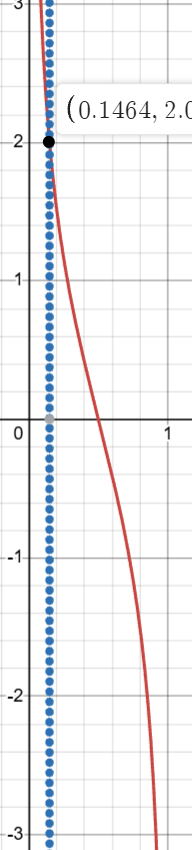
\includegraphics[width=0.2\textwidth]{Graph1c.png}
    \caption{Graph}
    \label{fig:myimage}
\end{figure}

We know that diffusitivity of a cable is proportional to the diameter. Looking
at the equation above, we now see that $c\propto \sqrt{d}$ which is the scaling.
So now if a neuron is mylenated, then the diameter of the neuron increases which
then increases the propogation speed. Since the speed is faster we don't have to 
initiate an action potential as much. (?)

\section{Question 2: Conductance-based synapses, shunting, and NMDA nonlinearity}

\textbf{a)} Rewriting the equation with the given constants and solving. We will also define
$\bar{g} = g_eE_e + g_iE_i + g_LE_L$.

\begin{align}
    C \frac{dV}{dt} &= -(g_L+g_e+g_i)V + (g_eE_e + g_iE_i + g_LE_L)\\
    C \frac{dV}{dt} +(g_L+g_e+g_i)V &=  \bar{g}\\
    \frac{dV}{dt} +\frac{(g_L+g_e+g_i)}{C}V &=  \frac{\bar{g}}{C}\\
    \frac{d}{dt} Ve^{\frac{(g_L+g_e+g_i)t}{C}} &=  \frac{\bar{g}}{C}e^{\frac{(g_L+g_e+g_i)t}{C}}\\
    V &=  \frac{\bar{g}}{g_L+g_e+g_i} + C_1e^{-\frac{(g_L+g_e+g_i)t}{C}}\\
    V &=  \frac{\bar{g}}{g_L+g_e+g_i} + C_1e^{\frac{-t}{\tau}}\\
\end{align}

Calculating steady state we get
\begin{align}
    0 &= -(g_L+g_e+g_i)V + (g_eE_e + g_iE_i + g_LE_L)\\
    V &=\frac{g_eE_e + g_iE_i + g_LE_L}{g_L+g_e+g_i}\\
\end{align}

with a time constant of $\tau = \frac{C}{g_L+g_e+g_i}$ and we can clearly see that
it relaxes exponentially to the conductance weighted average. Using
the given constants, we get a time constant of 
\begin{align}
    \tau_r = \frac{200*10^-12}{(10)*10^{-9}} = 20*10^{-3} = 20ms\\
    \tau_b = \frac{200*10^-12}{(40 + 10)*10^{-9}} = 4*10^{-3} = 4ms\\
\end{align}

Assuming no spiking when we have a fixed current:
\begin{align}
    0 &= -(g_L+g_e+g_i)V + \bar{g} + I\\
    V &=\frac{\bar{g} + I}{g_L+g_e+g_i}\\
    \implies V_r &= E_L + \frac{I}{10*10^{-9}}\\
    \implies V_b &= \frac{\bar{g}}{50*10^{-9}} + \frac{I}{50*10^{-9}}\\
\end{align}
In other words, when there is bombardment, the impact of the current on the 
voltage is lessened. Additionally, the time constant is smaller during bombardment
so the neuron will reach steady state faster.


\textbf{b)} Again calculating steady state by setting the change in voltage to 0 based on the equations from 2a, note that
voltage remains the same.
\begin{align}
    \implies V_r &= \frac{g_LE_L}{g_L} = E_L\\
    \implies V_i &= \frac{g_iE_i + g_LE_L}{g_i+g_L}\\
    &= \frac{g_iE_L + g_LE_L}{g_i+g_L}\\
    &= \frac{E_L(g_i + g_L)}{g_i+g_L} = E_L\\
\end{align}

If we include current, we can see below that the conductance of the inhibitory input
reduces the impact of I on voltage divisively.
\begin{align}
    \implies V_r &= \frac{g_LE_L + I}{g_L} = E_L + \frac{I}{g_L}\\
    \implies V_i &= \frac{g_iE_i + g_LE_L + I}{g_i+g_L}\\
    &= \frac{g_iE_L + g_LE_L + I}{g_i+g_L}\\
    &= \frac{E_L(g_i + g_L) + I}{g_i+g_L} = E_L + \frac{I}{g_i+g_L}\\
\end{align}

Evaluating it with the given constnts and assuming there is pretty much no excitatory conductance.
We can see that having a denominator increasing from $10nS$ to $30nS$ is an increase by a factor of 3,
hence shunting has a gain reduction of .6667, or more concretely.
\begin{align}
    \Delta V_i &= \frac{I}{30 nS}\\
    &= \frac{I}{10 nS} \frac{1}{3}\\
    &= \Delta V_r \frac{1}{3}
\end{align}

(multiplying by 1/3 is a .67 reduction and I do not know how to word it more eloquently)

\textbf{c)} Taking the derivative
\begin{align}
    B(V) &= \left[1+ \frac{[Mg^{2+}]}{3.57}e^{-V/V_0}\right]^{-1}\\
    B'(V) &= \left[1+ \frac{[Mg^{2+}]}{3.57}e^{-V/V_0}\right]^{-2}\frac{[Mg^{2+}]}{V_03.57}e^{-V/V_0}\\
    &= B(V)^{2}\frac{B(V)^{-1}-1}{V_0}\\
    &= \frac{B(V)^{2}-B(V)}{V_0}\\
    &= \frac{B(1-B)}{V_0}
\end{align}

Now with this information we can use the chain rule to calculate the next derivative:

\begin{align}
    \frac{dI_N}{V} &= \bar{g}\left[B'(V)(V-E_n) + B(V)\right]\\
    &= \bar{g}\left[\frac{B(1-B)}{V_0}(V-E_n) + B\right]\\
    &= \bar{g}B\left[\frac{(1-B)(V-E_n)}{V_0} + 1\right]\\
\end{align}

Need to review how to calculate these numbers\dots


\section{Question 3: Inferring a Poisson Rate}

\textbf{a)} So if we want to do baysian inference, do some short math... Note for step 18,
the simplification is done because the CDF of a probability function is 1.

\begin{align}
    P(v|K) &= \frac{P(K|v)P(v)}{P(K)}\\
    &= \frac{ \left(\frac{(vT)^Ke^{-vT}}{K!}\right) \left(\frac{b^a}{\Gamma(a)}v^{a-1}e^{-bv}\right)}
    {
        \frac{T^K}{K!}
        \frac{b^a\Gamma(a+K)}{\Gamma(a)(b+T)^{(a+K)}}
        \int_{0}^{\infty} \frac{(b+T)^{(a+K)}}{\Gamma(a+K)} v^{(a+K)-1} e^{-(b+T)v}  dv
    }\\
    &=\frac{ v^Ke^{-vT} \left(v^{a-1}e^{-bv}\right)}
    {
        \frac{\Gamma(a+K)}{(b+T)^{(a+K)}}
        *1
    }\\
    &=\frac{(b+T)^{(a+K)}}{\Gamma(a+K)}v^{(a+K)-1}e^{-(b+T)v}\\
    &= \Gamma(a+K,b+T)
\end{align}

To calculate the maximum likelihood function for v, assume we have some K spikes. Take the
derivative of the log likelihood function and maximize K chance based on v.

\begin{align}
    P(K|v) &= \frac{(vT)^Ke^{-vT}}{K!}\\
    \mathcal{L} &= \ln{\frac{(vT)^K}{K!}}-vT\\
    &= \ln(v^K) - vT + \ln\left(\frac{T^K}{K!}\right)\\
    \implies \mathcal{L}' &= \frac{K}{v} - T = 0\\
    \implies v &= \frac{K}{T}
\end{align}

Additionally using the information given the mean is $\frac{a+K}{b+T}$, the standard deviation is
$\frac{a+K}{(b+T)^2}$, and I assume the mode is the most likely to occur at the max of the gamma function but not sure how to calculate.

\textbf{b)} For this proof I will begin by working backwards. Also note that the prior mean is 
$a/b$ and the MLE is $K/T$
\begin{align}
    E[P(v|K)] &= \frac{a+K}{b+T}\\
    &= \frac{a}{b+T} + \frac{K}{b+T}\\
    &= \frac{b}{b+T} \frac{a}{b} + \frac{T}{b+T} \frac{K}{T}\\
\end{align}

Note the above equation is a weighted average of the prior and the MLE.

Based on the expected value of the prior, a is how many spikes occured and b is how long it took.

We know that $a = E[\text(prior)] * b= 5 *2 = 10$
\begin{align}
    MLE &= \frac{K}{T} = \frac{30}{3} = 10Hz\\
    Mean &= \frac{a+K}{b+T} = \frac{10 + 30}{2+3} = 8\\
    Var & = \frac{a+K}{(b+T)^2} = \frac{10 + 30}{(2+3)^2} = 1.6\\
    SD & = \sqrt{1.6} = 1.2649\\
\end{align}

If we want to halve the standard deviation, and I am going to assume spikes remain the same rate as measured.
We will solve for some $T'$ being additional time
\begin{align}
    \frac{1}{2}SD &= \frac{\sqrt{a+(K + 10T')}}{b+T+T'}\\
    0.63245 &= \frac{\sqrt{40 + 10T'}}{5+T'}\\
    0.63245(5+T') &= \sqrt{40 + 10T'}\\
    0.63245^2(5+T')^2 &= 40 + 10T'\\
    0.63245^2(T'^2+10T'+25)-40-10T' &= 0\\
    .4T'^2 -6T'-30 &= 0\\
    \implies T' &= \frac{6+ \sqrt{36+48}}{.8} = 18.9564\\
\end{align}

Hence it needs to be run for an additional $18.9564$ seconds.

\section{Question 4: Shot noise, balance, and diffusion approximation}

\textbf{a)} So the delta function is a weird function, so we will simply look at each step
and ensure continuity.

\begin{align}
    \tau \frac{dV}{dt} &= -V\\
    \frac{dV}{dt} + \frac{V}{\tau} &= 0\\
    \frac{d}{dt}Ve^{t/\tau} &= 0\\
    V &= Ce^{-t/\tau}
\end{align}
Looking at the step function.

Since we want to keep the decay condition while also allowing for a spike

\begin{align}
    V(t_1^+) - V(t_1^-) = w\\
    V(t_1^-) &= 0\\
    V(t_1^+) &= w\\
    \implies V &= we^{-(t-t_1)/\tau}
\end{align}

However say we have a second event then it would turn into
\begin{align}
    V(t_2^+) - V(t_2^-) &= w\\
    V(t_2^-) &= we^{-(t_2-t_1)/\tau}\\
    V(t_2^+) &= w + we^{-(t_2-t_1)/\tau}\\
    \implies V &= we^{-(t-t_1)/\tau} + we^{-(t-t_2)/\tau}
\end{align}

Hence if we keep summing up the impulses like this
\begin{align}
    V = w \sum_{k=1}^K e^{-(t-t_k)/\tau}
\end{align}

Now if we divide it into widths of ds, with events occurring independnetally with probability vds.
Define this random variable as $X_j$ then we get the following.


\begin{align}
    V = w \sum_{j} X_i e^{-(t-s_j)/\tau}
\end{align}

Note for the above we used $s_j$ as this makes it much nicer to solve other stuff where s is time.
Additionally we assume t is the current state we are at and it is the steady state. Additionally
$X_j$ is bernoulli.

\begin{align}
    <V> &= w \sum_{j} <X_i> e^{-(t-s_j)/\tau}\\
    &= w \sum_{j} vds e^{-(t-s_j)/\tau}\\
    &= wv \int_{-\infty}^{t}e^{-(t-s)/\tau}ds\\
    &= wv \left[\tau e^{-(t-s)/\tau}\right]|_{-\infty}^t\\
    &=wv\tau\\
    Var(V) &= Var\left[w\sum_{j} X_i e^{-(t-s_j)/\tau}\right]\\
    &= w^2\sum_{j} Var\left[X_i e^{-(t-s_j)/\tau}\right]\\
    &= w^2\sum_{j} e^{-2(t-s_j)/\tau}Var\left[X_i \right]\\
    &= w^2\sum_{j} e^{-2(t-s_j)/\tau}(vds)(1-vds)\\
    &\approx w^2\sum_{j} e^{-2(t-s_j)/\tau}vds\\
    &= w^2v\int_{-\infty}^t e^{-2(t-s)/\tau}ds\\
    &= w^2v\frac{\tau}{2}  \left[e^{-2(t-s)/\tau}\right|_{-\infty}^t\\
    &= \frac{vw^2\tau}{2}
\end{align}

\textbf{b)} 

Rewriting the equation we get something similar to the equation below 
\[
P(X_j = x) = \begin{cases}
    v_E & 1\\
    1-v_E & 0
\end{cases}
\]

\[
P(Y_j = y) = \begin{cases}
    v_I & 1\\
    1-v_I & 0
\end{cases}
\]

\begin{align}
    V = w \sum_{j} (X_j - Y_j) e^{-(t-s_j)/\tau}
\end{align}

To make it easier to calculate split up the terms, and by using the property of independence
\begin{align}
    V &= w \sum_{j} X_j e^{-(t-s_j)/\tau} -w \sum_{j} Y_je^{-(t-s_j)/\tau}\\
    <V> &= <w \sum_{j} X_j e^{-(t-s_j)/\tau}> - <w \sum_{j} Y_je^{-(t-s_j)/\tau}>\\
    &= (v_E-V_I)w\tau\\
    Var(V) &= Var(w \sum_{j} X_j e^{-(t-s_j)/\tau}) + Var(w \sum_{j} Y_je^{-(t-s_j)/\tau})\\
    &= \frac{(v_E+v_I)w^2\tau}{2}
\end{align}
Note since you square a constant when it is taken out of a variance operation as done in (175), you end up with only sums.
Hence if the rate of inhibition and excitation is the same, they cancel each other out in the mean, but
as they increase, the variance also increases.

Now if we use the constants that were given

\begin{align}
    <V> &= .01(v_E-v_I) = 10\\
    Var(V) &= \frac{.005(v_E+v_I)}{2} = 25\\
    \implies v_E+v_I &= 10000\\
    \implies v_E-v_I &= 1000\\
    \implies v_E &= 5500\\
    \implies v_I &= 4500\\
\end{align}

I don't really know what this says about the active synapse, but if we assume that all synapse
have the same chance of firing, then there are more excitatory synapses then inhibitory synapses.

\textbf{c) + d)} I do not know how to do math regarding cumulants.

\section{Question 5) Stationary Density and Firing Rate of a noisy Integrator}

Not Completed


\end{document}